%%
%% $Id: article.tex,v 1.1 2008/09/20 10:19:28 natalie Exp $
%% $Source: /Users/natalie/cvs/tex/templates/article.tex,v $
%% $Date: 2008/09/20 10:19:28 $
%% $Revision: 1.1 $
%%

%\documentclass[a4paper,11pt,BCOR1cm,DIV11,headinclude]{scrbook}
% bei 12pt ist DIV 12 default, bei 11pt ist es DIV 10
% Textbereiche 
% DIV 10: 147*207.9mm, DIV 11: 152.73*216mm, DIV 12:157.50*222.75
% DIV 13: 161.54*228.46mm, DIV 14: 165*233.36mm

\def\deftitle{Notes on hedging cryptos with spectral risk measures}
% \def\defauthor{N.\ Packham}
% \def\defauthor{nat}
\def\defauthor{}

%% option: largefont
\documentclass[square]{article} %
%% options: vscreen, garamond, wnotes, savespace
\usepackage[vscreen]{nat}
\usepackage[longnamesfirst]{natbib}
\bibpunct{(}{)}{;}{a}{,}{,}
\usepackage{amsfonts,amssymb,amsthm} %
\usepackage[tbtags]{amsmath} %
% \usepackage{fullpage}

\usepackage{graphicx,color}
\graphicspath{{./pics/}}
\definecolor{BrickRed}{rgb}{.625,.25,.25}
\providecommand{\red}[1]{\textcolor{BrickRed}{#1}}
\definecolor{markergreen}{rgb}{0.6, 1.0, 0}
\definecolor{darkgreen}{rgb}{0, .5, 0}
\definecolor{darkred}{rgb}{.7,0,0}
\providecommand{\marker}[1]{\fcolorbox{markergreen}{markergreen}{{#1}}}
\providecommand{\natp}[1]{\textcolor{darkred}{#1}}
\theoremstyle{plain}
\newtheorem{theorem}{Theorem}%[section]
\newtheorem{proposition}[theorem]{Proposition}
\newtheorem{corollary}[theorem]{Corollary} %%
\newtheorem{lemma}[theorem]{Lemma} %%
\theoremstyle{definition} %%
\newtheorem{definition}{Definition}
\newtheorem{remark}[theorem]{Remark}
\newtheorem{remarks}{Remarks}
\newtheorem{condition}[theorem]{Condition}
\newtheorem{example}[theorem]{Example}
\newtheorem{assumption}{Assumption}

\usepackage[makestderr]{pythontex}
\usepackage{amsmath}
\begin{pycode}
import numpy as np
from scipy import stats
import statsmodels.api as sm
import pandas as pd
import matplotlib.pyplot as plt
np.random.seed(87654)
\end{pycode}


%%
%% $Id: Definitions.tex,v 1.6 2008/07/26 14:55:50 natalie Exp $
%% $Source: /Users/natalie/cvs/tex/dynamics/Definitions.tex,v $
%% $Date: 2008/07/26 14:55:50 $
%% $Revision: 1.6 $
%%

%\usepackage{mathrsfs}

%% GENERAL DEFINITIONS
\unitlength1cm

%% COMMAND DEFINITIONS
\newcommand{\E}{{\mathbb{E}}}
%%\renewcommand{\E}{{\mathds E}}
%%\renewcommand{\E}{{\varmathbb{E}}}
%%\renewcommand{\E}{{\mathrm{I\!E}}}
\providecommand{\R}{{\mathbb{R}}}
\newcommand{\T}{{\mathbb{T}}}
\newcommand{\Fb}{{\mathbb{F}}}
\newcommand{\Eqn}{{\mathbb{E}}_{{\bf Q}_N}}
\newcommand{\Eq}{{\mathbb{E}}_{{\bf Q}}}
\newcommand{\Eqm}{{\mathbb{E}}_{{\bf Q}_M}}
\newcommand{\EqT}{{\mathbb{E}}_{{\bf Q}_T}}
\newcommand{\EqTz}{{\mathbb{E}}_{{\bf Q}_{T_2}}}
\newcommand{\EqTe}{{\mathbb{E}}_{{\bf Q}_{T_1}}}
\newcommand{\EqSe}{{\mathbb{E}}_{{\bf Q}_{S^1}}}
\newcommand{\EqSz}{{\mathbb{E}}_{{\bf Q}_{S^2}}}
\newcommand{\p}{{\bf P}}
%%\renewcommand{\p}{{\mathds{P}}}
%%\renewcommand{\p}{{\varmathbb{P}}}
%%\renewcommand{\p}{{\mathrm{I\!P}}}
\newcommand{\pas}{\text{{\bf P}--a.s.}}
\newcommand{\paa}{\text{{\bf P}--a.a.}}
\newcommand{\qas}{\text{{\bf Q}--a.s.}}
\newcommand{\e}{{\bf e}}
\newcommand{\q}{{\bf Q}}
\newcommand{\qn}{{\bf Q}_N}
\newcommand{\qm}{{\bf Q}_M}
\newcommand{\qT}{{\bf Q}_T}
\newcommand{\qTz}{{\bf Q}_{T_2}}
\newcommand{\qTe}{{\bf Q}_{T_1}}
\newcommand{\qS}{{\bf Q}_S}
\newcommand{\qSe}{{\bf Q}_{S^1}}
\newcommand{\qSz}{{\bf Q}_{S^2}}
\newcommand{\F}{{\cal F}}
\newcommand{\G}{{\cal G}}
\newcommand{\A}{{\cal A}}
\newcommand{\Hc}{{\cal H}}
\newcommand{\dP}{{\rm d}{\bf P}}
\newcommand{\du}{{\rm d}u}
%%\newcommand{\dt}{{\rm d}t}
\newcommand{\dd}{{\rm d}}
\newcommand{\df}{{\rm \bf DF}}
\providecommand{\N}{{\mathbb N}}
\providecommand{\Ncdf}{{\rm N}}
%\renewcommand{\Ncdf}{{\Phi}}
\newcommand{\n}{{\rm n}}
\newcommand{\emb}{\bf \em}
\newcommand{\1}{\textbf{1}}
\newcommand{\qs}{{\q_{\rm Swap}}}
\newcommand{\fx}{{\rm fx}}
\newcommand{\V}{{\rm Var}}
%\newcommand{\C}{{\bf C}}
\newcommand{\Om}{{\Omega}}
\providecommand{\limn}{\ensuremath{\lim_{n\rightarrow\infty}}}
\providecommand{\qv}[2]{\ensuremath{\langle #1,#1\rangle_{#2}}}

%% ENVIRONMENT DEFINITIONS
%\newtheorem{prop}{Proposition}[section]
%\newtheorem{theo}{Theorem}[section]
%\newtheorem{lem}{Lemma}[section]
%\newtheorem{ass}{Assumption}[section]
%\newtheorem{cor}{Corollary}[section]
%\newtheorem{aufg}{Exercise}[section]
%\newtheorem{defi}{Definition}[section]

\ifx\prop\undefined
\newtheorem{prop}{Proposition}[section]
\fi
\newtheorem{theo}[prop]{Theorem}
\newtheorem{lem}[prop]{Lemma}
\newtheorem{cor}[prop]{Corollary}
\newtheorem{defi}[prop]{Definition}

%% enumeration in lists
\providecommand{\labelenumi}{{\rm (\roman{enumi})}}
   %\setlength{\topsep}{0cm}
    \setlength{\labelsep}{0.3cm}
    %\setlength{\itemindent}{0cm}
   \setlength{\leftmargin}{10cm}
    \setlength{\labelwidth}{5cm}

\providecommand{\cadlag}{c\`adl\`ag }
\providecommand{\cadlagns}{c\`adl\`ag}
\providecommand{\caglad}{c\`agl\`ad }
\providecommand{\cad}{c\`ad}
\providecommand{\cag}{c\`ag}
\providecommand{\levy}{L\'evy\ }
\providecommand{\levyns}{L\'evy}
\providecommand{\levyito}{L\'evy-It\^o\ } 
\providecommand{\levykhinchin}{L\'evy-Khinchin\ }
\providecommand{\D}{\ensuremath{D(\R_+,\R)}}
\providecommand{\Dsig}{\ensuremath{D(\R_+, \R_+\setminus\{0\}})}
\providecommand{\Dd}{\ensuremath{D(\R_+,\R^d)}}
\providecommand{\C}{\ensuremath{C(\R_+,\R)}}
\providecommand{\Cd}{\ensuremath{C(\R_+,\R^d)}}
\providecommand{\rpos}{\ensuremath{{[0,\infty)}}}

\def\Z{{\mathbb Z}}
%\def\N{{\mathbb N}}
%\def\R{{\mathbb R}}
%\def\C{{\mathbb C}}
%\def\H{{\mathbb H}}
\def\P{{\mathbb P}}
\def\Q{{\mathbb Q}}
%\def\E{{\mathbb E}}
\def\I{{\mathbb I}}
%\def\T{{\mathbb T}}
%\def\F{{\mathbb F}}
\def\M{{\mathbb M}}
%\def\Hc{{\mathcal H}}
\def\Mc{{\mathcal M}}
\def\filtration#1{{\ensuremath\mathcal{#1}}}
%\def\filt{{\mathcal F}}
\def\tp{\tilde{\p}}
\providecommand{\vec}[1]{\ensuremath{\bm #1}}
\providecommand{\vecb}[1]{\ensuremath{\bm #1}}
\providecommand{\abs}[1]{\ensuremath{\lvert#1\rvert}}
\providecommand{\norm}[1]{\ensuremath{\lVert#1\rVert}}
\providecommand{\var}{\ensuremath{\text{Var}}}
\providecommand{\cov}{\ensuremath{\text{Cov}}}
\providecommand{\borel}[0]{\ensuremath{\mathcal{B}}}
\providecommand{\intinf}[0]{\ensuremath{\int_{-\infty}^\infty}}
\providecommand{\intpos}[0]{\ensuremath{\int_0^\infty}}
\providecommand{\intneg}[0]{\ensuremath{\int_{-\infty}^0}}
\providecommand{\todo}[1]{\footnote{#1}}
\providecommand{\dynkin}[0]{\ensuremath{\mathcal D}}
\providecommand{\ce}[2]{\ensuremath{\E(#1|\filtration{#2})}}
\providecommand{\inv}[1]{\ensuremath{#1^{(-1)}}}
\providecommand{\os}[2]{\ensuremath{#1^{(#2)}}}
\providecommand{\pos}[2]{\ensuremath{h_{#1}(#2)}}
%\providecommand{\poslong}[2]{\ensuremath{h(#1, #2)}}
\providecommand{\poslong}[3]{\ensuremath{h_{#1, #2}(#3)}}

%% Class of finite variation processes
\providecommand{\classfv}{\ensuremath{\mathscr V}}
\providecommand{\classv}{\ensuremath{\mathscr V}}
%% Stochastic integral operator
\providecommand{\stint}{\ensuremath{\cdotp}}
\providecommand{\classh}{\ensuremath{\mathscr H^2}}
\providecommand{\classhloc}{\ensuremath{\mathscr H^2_{\rm loc}}}
\providecommand{\classm}{\ensuremath{\mathscr M}}
\providecommand{\classmloc}{\ensuremath{\mathscr M_{\rm loc}}}
\providecommand{\classl}{\ensuremath{L^2}}
\providecommand{\classlloc}{\ensuremath{L^2_{\rm loc}}}
\providecommand{\classa}{\ensuremath{\mathscr A}}
\providecommand{\classaloc}{\ensuremath{\mathscr A_{\rm loc}}}
\providecommand{\classalocpos}{\ensuremath{\mathscr A_{\rm loc}^+}}
\providecommand{\classp}{\ensuremath{\mathscr P}}
\providecommand{\classo}{\ensuremath{\mathscr O}}
\providecommand{\classs}{\ensuremath{\mathscr S}}
\providecommand{\classsp}{\ensuremath{\mathscr S_p}}
\providecommand{\nullset}{\ensuremath{\mathscr N}}

\providecommand{\ito}{It\^o }
\providecommand{\itos}{It\^o's\, }

\providecommand{\variation}[2]{\ensuremath{\rm V_{#1}(#2)}}
\renewcommand{\H}{\ensuremath{\mathcal H}}
%% CPO distribution
\providecommand{\cpo}{\ensuremath{{\rm CPO}}}
\providecommand{\Fsigma}{\ensuremath{\mathcal \F_\infty^\sigma}}
\providecommand{\sigd}{\ensuremath{\mathscr D}}

%% Credit spreads
\providecommand{\s}{{\bf s}}
\providecommand{\classu}{\ensuremath{\mathscr U}}

\providecommand{\sX}{\ensuremath{\mathcal X}}
\providecommand{\sY}{\ensuremath{\mathcal Y}}
\providecommand{\dx}{\ensuremath{\frac{\partial}{\partial x}}} %%
\providecommand{\dt}{\ensuremath{\frac{\partial}{\partial t}}} %%
\providecommand{\dy}{\ensuremath{\frac{\partial}{\partial y}}} %%
\newcommand{\argmax}{\operatornamewithlimits{argmax}}
\newcommand{\argmin}{\operatornamewithlimits{argmin}}

\sloppy
\begin{document}
\setlength{\boxlength}{0.95\textwidth} %
\title{\large{\bf\deftitle}} %
\author{{\normalsize\bf\defauthor}}%
\thispagestyle{empty}
\addtocounter{page}{1}
\maketitle
\begin{abstract}
  We investigate different methods of hedging cryptocurrencies with
  Bitcoin futures. A useful generalisation of variance-based hedging
  uses spectral risk measures and copulas. 
\end{abstract}
% \keywords{keywords here} %%
% \jel{jel here} %%
\vspace{.5cm}
\def\contentsname{Contents}
\tableofcontents
%%
\vspace{.5cm}
%\clearpage

\section{Optimal hedge ratio}
\label{sec:optimal-hedge-ratio}

Following \citep{Barbi2014}, we consider the problem of the optimal
hedge ratios by extending commmonly known minimum variance hedge ratio
to more general risk measures and dependence structures.\medskip\\
Hedge portfolio: $R_t^h = R_t^S - h R_t^F$, involving returns of spot
and future contract and where $h$ is the hedge ratio\\
Optimal hedge ratio: $h^\ast = \argmin_h \rho_\phi(s,h)$, for given
confidence level $1-s$ (if applicable, e.g.\ in the case of VaR, ES),
where $\rho_\phi$ is a spectral risk measure with weighting function
$\phi$ (see below). \\ 
Corollary 2.1 of \citep{Barbi2014}, corrected: Let $R^S$ and $R^F$ be
two real-valued random variables on the same probability space
$(\Omega, \mathcal A, \p)$ with corresponding absolutely continuous
copula $C^t_{R^S, R^F}(w,\lambda)$ and continuous marginals $F_{R^S}$
and $F_{R^F}$. Then, the $s$-quantile of $R^h$ solves the following:
\begin{equation*}
  F_{R^h}(r^h) = 1- \int^1_0 D_1 C_{R^S, R^F}
  \left\{ w, F_{R^F} \left[ \frac{F^{-1}_{R^S}(w)-r^h}{h} \right]
  \right\}dw.  
\end{equation*}
[..]\\
Here $D_1 C(u,v)=\displaystyle \frac{\partial}{\partial u} C(u,v)$,
which can be shown to fulfil \citep{Cherubini2011}
\begin{equation*}
  D_1 C_{X,Y}(F_X(x), F_Y(y)) = \p(Y\leq y|X=x).
\end{equation*}

\section{Spectral risk measures}
\label{sec:spectr-risk-meas}

Spectral risk measure \citep{Acerbi2002,Cotter2006}:
\begin{equation*}
\rho_\phi = -\int_0^1 \phi(p)\, q_p\, \dd p,
\end{equation*}
where $q_p$ is the $p$-quantile of the return distribution and
$\phi(s)$, $s\in [0,1]$, is the so-called {\em risk aversion
  function\/}, a weighting function such that\footnote{Note that the
  treatment in \citep{Acerbi2002} is measure-based and therefore
  slightly different} 
\begin{enumerate}[(i)]
\item $\phi(p)\geq 0$,
\item $\int_0^1\phi(p)\, \dd p=1$,
\item $\phi'(p)\leq 0$. 
\end{enumerate}
Examples: VaR, ES\\
Replacing the last property with $\phi'(p)>0$ rules out risk-neutral
behaviour. \\
Spectral risk measures are coherent \citep{Acerbi2002}. 

\subsection{Representation of spectral risk measures}
\label{sec:repr-spectr-risk}

To prevent numerical instabilities involving the quantile function,
re-write spectral risk measures as follows:
\begin{itemize}
\item Integration by substitution: $\displaystyle \int_a^b
  g(\varphi(x)) \,\varphi'(x)\, \dd x = \int_{\varphi(a)}^{\varphi(b)}
  g(u)\, \dd u$.
\item Spectral risk measures: $\displaystyle -\int_0^1 \phi(p) \,
  F^{(-1)}(p)\, \dd p$
\item Set $\varphi(x)=F(x)$, $g(p) = \phi(p)\, F^{(-1)}(p)$.
\item Then:
  \begin{equation*}
    -\int_0^1 \phi(p)\, F^{(-1)}(p)\, \dd p = -\int_{-\infty}^\infty
    \phi(F(x))\, x\, f(x)\, \dd x.
  \end{equation*}
\end{itemize}


\subsection{Exponential spectral risk measures}
\label{sec:expon-risk-meas}

\begin{itemize}
\item Choose exponential utiliy function:
  $\displaystyle U(x) = -\e^{-k x}$, where $k>0$ is the Arrow-Pratt
  coefficient of absolute risk aversion
  (ARA).
\item Coefficient of absolute risk aversion: $\displaystyle R_A(x) =
  -\frac{U''(x)}{U'(x)} = k$
\item Coefficient of relative risk aversion: $\displaystyle R_R(x) = -
  \frac{x U''(x)}{U'(x)} = xk$
\item Weighting function $\phi(p) = \lambda \e^{-k(1-p)}$, where
  $\lambda$ is an unknown positive constant.
\item Set $\displaystyle\lambda = \frac{k}{1-\e^{-k}}$ to satisfy
  normalisation.
\item Exponential spectral risk measure:
  \begin{equation*}
    \rho_{\phi} = \int_0^1 \phi(p)\, F^{(-1)}(p)\, \dd p =
    \frac{k}{1-\e^{-k}} \int_0^1 \e^{-k(1-p)}\, F^{(-1)}(p)\, \dd p. 
  \end{equation*}
(If calculation of quantiles is a problem use change of variables
above.)
\item What exactly is the link between risk measure and utility?
    I think there is no direct link: the exponential risk measure is
   {\em inspired\/} by ARA utility.
\end{itemize}


%! Author = francis
%! Date = 30.10.20

\section{$D_1$ Operator}

The $D_1$ operator is given as
\begin{equation*}
    D_1 C_{X,Y}(F_X(x), F_Y(y)) = \p(Y\leq y|X=x).
\end{equation*}
In the context of the above notation, we obtain
\begin{align*}
  D_1 C_{R^s, R^F}(w, g(w)) &= \p(R_F\leq F_{F}^{(-1)}(g(w))|
  R_s=F_S^{(-1)}(w)) %
  = \p(V\leq g(w)| U=w)\\ %
  &= \frac{\p(U\in \dd w, V\leq g(w))} {\p(U\in \dd w)} %
  = \p(U\in \dd w| V\leq g(w)) %
  = \int_0^{g(w)} c(w,v)\, \dd v. 
\end{align*}
The last line can also be written as
\begin{equation*}
  \frac{\partial }{\partial w} C(w, g(w')) \big|_{w'=w}. 
\end{equation*}



We give an explicit equation of the $D_1$ operator for Archimedean copulae.

The $D_1$ operator is defined as the partial derivatives of the first input to the copula function,
so we fix the second argument while taking derivative with respect to the first, and then evaluate the function.
we have

\begin{align}
\left.\frac{\partial C\{v, g(w)\}}{\partial v} \right\vert_{v=w}
&=
\left.\frac{\partial  \phi^{-1}[\phi(v)+\phi\{g(w)\}]}
{\partial  [\phi(v)+\phi\{g(w)\}]}
\frac{\partial  [\phi(v)+\phi\{g(w)\}]}
{\partial  v}
\right\vert_{v=w}\\
&=
\left.\frac{\partial   \phi^{-1}[\phi(v)+\phi\{g(w)\}]}
{\partial [\phi(v)+\phi\{g(w)\}]}
\frac{\partial  \phi(v)}{\partial  v}
\right\vert_{v=w}\\
&=
\frac{\partial \phi^{-1}[\phi(w)+\phi\{g(w)\}]}
{\partial [\phi(w)+\phi\{g(w)\}]}
\frac{\partial  \phi(w)}{\partial  w}\\
&,
\text{where } g(w) = F_{R^F}\left\{\frac{F^{-1}_{R^S}(w)-r^h}{h}\right\}\\
\end{align}

\begin{table}
    \center
    \begin{tabular}{c c c c c}
        Function & Gumbel & Frank & Clayton & Independence\\
        $\phi(t)$    &
        $\{-\log(t)\}^\theta$ &
        $-\ln \left\{
        \frac{\exp(-\theta t)-1}
        {\exp(-\theta)-1}
        \right\}$&
        $\frac{1}{\theta}
        (t^{-\theta}-1)$
        & Same to Gumbel where $\theta=1$\\
        $\phi^{-1}(t)$ &
        $\exp(-t^{1/\theta})$ &
        $\frac{-1}{\theta}
        \log[1+ \exp(-t)\{\exp(-\theta)-1\}]$ &
        $(1+\theta t)^{-\frac{1}{\theta}}$
        & \\

        $\partial \phi(t)/\partial t$ &
        $\theta \frac{\phi(t)}{t\log(t)}$ &
        $\frac{\theta \exp(-\theta t)} {\exp(-\theta t)-1}$ &
        $-t^{-(\theta + 1)}$&
        \\
        $\partial \phi^{-1}(t)/\partial t$ &
        $\frac{-1}{\theta}t^{\frac{1}{\theta}-1}\phi^{-1}(t)$&
        $\frac{1}{\theta}\frac{\exp(-t)\{\exp(-\theta)-1\}}{1+\exp(-t)\{\exp(-\theta)-1\}}$&
        $\theta (1+\theta t)^{-\frac{1}{\theta}-1}$&
        \end{tabular}\label{tab:archcopula}
\end{table}








\section{Dependence}
\label{sec:dependence}

Dependence through copula (e.g.\ Student t, Clayton or Gumbel)

\subsection{Archimedean copulas}
\label{sec:archimedean-copulas}

\begin{itemize}
\item A well-studied one-parameter family of copulas are the {\bf 
    Archimedean copulas}. 
\item Let $\phi:[0,1]\rightarrow[0,\infty]$ be a
  continuous and strictly decreasing function with $\phi(1)=0$ and
  $\phi(0)\leq\infty$.
\item  We define the {\bf pseudo-inverse} of $\phi$ as 
  \begin{equation*}
    \phi^{(-1)}(t)=
    \begin{cases}
      \phi^{-1}(t), &0\leq t\leq \phi(0),\\
      0, &\phi(0)<t\leq\infty.
    \end{cases}
  \end{equation*}
\item If, in addition, $\phi$ is convex, then the following function
  is a copula: 
  \begin{equation*}
    C(u,v)=\phi^{(-1)}(\phi(u)+\phi(v)).
  \end{equation*}
  \vspace*{-\baselineskip}
\item Such copulas are called {\bf Archimedean copulas}, and the
  function $\phi$ is called an {\bf Archimedean copula generator}. 
\item Examples of Archimedean copulas are the {\bf Gumbel} and the
  {\bf Clayton} copulas:
  \begin{align*}
    C_{\theta,{\rm Gu}}(u,v) &= \exp\left\{-((-\ln u)^\theta + (-\ln
                               v)^\theta)^{1/\theta}\right\},& 1\leq \theta<\infty,\\
    C_{\theta,{\rm Cl}}(u,v)&= (u^{-\theta} + v^{-\theta}
                              -1)^{-1/\theta}, & 0<\theta<\infty. 
  \end{align*}
\item In the case of the Gumbel copula, the independence copula is 
  attained when $\theta=1$ and the comonotonicity copula is attained
  as $\theta\rightarrow\infty$. 
\item Thus, the Gumbel copula interpolates between independence and
  perfect dependence.  
\item In the case of the Clayton copula, the independence copula is
  attained as $\theta\rightarrow 0$, whereas the comonotonicity
  copula is attained as $\theta\rightarrow\infty$. 
\end{itemize}


\section{Estimation}
%! Author = francis
%! Date = 30.10.20


\subsection{Simulated Method of Moments}\label{subsec:simulated-method-of-moments}
This method is suggested by Oh and Patton (2013).
In this setting, rank correlation e.g. Spearman's $\rho$ or Kendall's $\tau$,
and quantile dependence measures at different levels $\lambda_q$
are calibrated against their empirical counterparts.\medskip

Spearman's rho, Kendall's tau, and quantile dependence of a pair $(X,Y)$
with copula $C$ are defined as
\begin{align}
  \rho_S &= 12 \int\int_{I^2} C_{\bm{\theta}}(u,v)\, \dd u\, \dd v-3\label{eq:rho_S}\\
  \tau_K &= 4\mathbb{E}[C_{\bm{\theta}}\{F_X(x), F_Y(y)\}]-1,\\
  \lambda_q &=
  \begin{cases}
    \p(F_X(X)\leq q| F_Y(Y)\leq q) = \displaystyle \frac{C_{\bm{\theta}}(q,q)}{q},
    &\text{ if } q\in (0,0.5],\\
    \p(F_X(X)>q|F_Y(Y)>q) =\displaystyle \frac{1-2q+C_{\bm{\theta}}(q,q)} {1-q},
    &\text{ if } q\in (0.5,1).
  \end{cases}
\end{align}\medskip
The empirical counterparts are
\begin{align*}
  \hat\rho_S &= \frac{12}{n} \sum_{k=1}^n \hat F_X(x_k) \hat F_Y(y_k)
               -3,\\
  \hat\tau_K &= \frac{4}{n}\sum_{k=1}^n \hat{C}\{\hat{F}_X(x_i),\hat{F}_X(y_i)\} -1 ,\\
  \hat\lambda_q &=
                  \begin{cases}
                    \displaystyle\frac{1}{n} \sum_{k=1}^n \frac{\1_{\{\hat
                        F_X(x_k)\leq q, \hat F_Y(y_k)\leq q\}}} {q},
                    &\text { if } q\in (0, 0.5],\\
                    \displaystyle \frac{1}{n} \sum_{k=1}^n
                    \frac{\1_{\{\hat F_X(x_k)>q, \hat F_Y(y_k)>q\}}}
                    {1-q}, &\text { if } q\in (0.5,1).
                  \end{cases},
\end{align*}
where $\hat{F}(x) := \frac{1}{n}\sum_{k=1}^n 1_{\{x_i\leq x\}}$ and
$\hat{C}(u,v) := \frac{1}{n}\sum_{k=1}^n 1_{\{u_i\leq u, v_i\leq v\}}$.\medskip

We denote $\tilde{\bm{m}}(\bm{\theta})$ be a $m$-dimensional vector of dependence measures according the the
dependence parameters $\bm{\theta}$,and  $\hat{\bm{m}}$ be the corresponding empirical counterpart.
The difference between dependence measures and their counterpart is denoted by
\begin{align*}
    \bm{g}(\bm{\theta}) = \hat{\bm{m}} - \tilde{\bm{m}}(\bm{\theta}).
\end{align*}\medskip

The SMM estimator is
\begin{align*}
    \hat{\bm{\theta}} = \argmin_{\bm{\theta}\in \bm{\Theta}} \bm{g}(\bm{\theta})^\intercal
    \hat{\bm{W}}
     \bm{g}(\bm{\theta}),
\end{align*}
where $\hat{W}$ is some positive definite weigh matrix.\medskip

In this work, we use $\tilde{\bm{m}}(\bm{\theta}) = (\rho_S, \lambda_{0.05}, \lambda_{0.1},
\lambda_{0.9}, \lambda_{0.95})^\intercal$
for calibration of Bitcoin price and CME Bitcoin future.

\subsection{Maximum Likelihood Estimation}\label{subsec:maximum-likelihood-estimation}
By Sklar's theorem, the joint density of a $d$-dimensional random variable $\bm{X}$ with sample size $n$ can be written as
\begin{align}
    \bm{f}_{\bm{X}}(x_1, ..., x_d) = \bm{c}\{F_{X_1}(x_1), ..., F_{X_d}(x_d)\} \prod_{j=1}^d f_{X_i}(x_i).
    \end{align}
We follow the treatment of MLE documented in section 10.1 of \citet{joe1997multivariate}, namely the inference functions for margins or IFM method.
The log-likelihood $\sum^n_{i=1}f_{\bm{X}}(X_{i,1}, ..., X_{i,d})$ can be decomposed into dependence part and marginal part,
\begin{align}
    L(\bm{\theta}) &= \sum_{i=1}^n \bm{c}\{F_{X_1}(x_{i,1};\bm{\delta}_1), ..., F_{X_d}(x_{i,d}; \bm{\delta}_d);\bm{\gamma}\}
    + \sum_{i=1}^n \sum_{j=1}^d f_{X_j}(x_{i,j};\bm{\delta}_j)
    &= L_C(\bm{\delta}_1, ..., \bm{\delta}_d, \bm{\gamma}) + \sum_{j=1}^d L_j(\bm{\delta}_j)
    \end{align}
where $\bm{\delta}_j$ is the parameter of the $j$-th margin, $\bm{\gamma}$ is the parameter of the parametric copula, and
$\bm{\theta} = (\bm{\delta}_1,..., \bm{\delta}_d, \bm{\gamma})$.

Instead of searching the $\bm{\theta}$ is a high dimensional space, \citet{joe1997multivariate} suggests to
search for $\hat{\bm{\delta}_1},..., \hat{\bm{\delta}_d}$ that maximize $L_1(\bm{\delta}_1), ..., L_d(\bm{\delta}_d)$,
then search for $\hat{\bm{\gamma}}$ that maximize $L_C(\hat{\bm{\delta}_1},..., \hat{\bm{\delta}_d}, \bm{\gamma})$.

That is, under regularity conditions, $(\hat{\bm{\delta}_1},..., \hat{\bm{\delta}_d}, \hat{\bm{\gamma}})$ is the solution of
\begin{align}
    \left( \frac{\partial L_1}{\partial \bm{\delta}_1}, ..., \frac{\partial L_d}{\partial \bm{\delta}_d},
    \frac{\partial L_C}{\partial \bm{\gamma}}\right) = \bm{0}.
    \end{align}

However, the IFM requires making assumption to the distribution of of the margins.
\citet{genest1995semiparametric} suggests to replace the estimation of marginals parameters estimation by non-parameteric estimation.
Given non-parametric estimator $\hat{F}_i$ of the margins $F_i$, the estimator of the dependence parameters $\bm{\gamma}$ is
\begin{align}
    \hat{\bm{\gamma}} = \argmax_{\bm{\gamma}} \sum_{i=1}^n \bm{c}\{ \hat{F}_{X_1}(x_{i,1}), ..., \hat{F}_{X_d}(x_{i,d});\bm{\gamma}\}.
    \end{align}



%With the decomposition, the MLE estimator for a bivariate parametric copula is
%\begin{align}
%    \hat{\bm{\theta}} = \argmax_{\bm{\theta} \in \bm{\Theta}} l(X_1,X_2; \bm{\theta}), \label{eq:EMLE}
%    \end{align}
%where
%\begin{align}
%    l(X_1,X_2; \bm{\theta}) = \sum_{i=1}^n \log c(x_{i,1}, x_{i,2};\bm{\theta}). \label{eq:Likelihood}
%    \end{align}\medskip

%Procedure of maximising equation~\ref{eq:EMLE} as a whole is called exact maximum likelihood method.
%Leveraging the attractive feature of copula that one can model the dependence structure and marginals separately,
%we rewrite~\ref{eq:Likelihood} into canonical expression
%\begin{align}
%    l(X,Y; \bm{\theta}) = \sum_{k=1}^n \log c\{F_X(x_i; \delta_X), F_Y(y_i; \delta_Y); \bm{\gamma}\}
%    + \sum_{k=1}^n \log f_X(x_i; \bm{\delta}_X) + \sum_{k=1}^n \log f_X(y_i; \bm{\delta}_Y),
%    \end{align}
%where the $\bm{\gamma}$ is the dependence parameter in the copula and $\bm{\delta}$ is the parameters in the margins.\medskip
%
%The inference-functions for margins (IFM) approach by Joe is a two step procedure of maximising~\ref{eq:EMLE}.
%The approach calibrate first the $\bm{\delta}$s and then the  $\bm{\gamma}$.\medskip
%
%Similar to the IFM approach, pseudo-maximum likelihood approach by Genest and Rivest (1993) replace the parametric margins by
%empirical estimates, we rewrite \ref{eq:Likelihood} again with
%\begin{align}
%    l(X,Y; \bm{\theta}) = \sum_{k=1}^n \log c(u_i, v_i;\bm{\gamma}),
%    \end{align}
%where $u_i = \hat{F}_X(x_i)$ and $v_i = \hat{F}_Y(y_i)$.

\subsection{Comparison}
Both the simulated method of moments and the maximum likelihood estimation are unbiased and
proven to give good fits.
The problem remain is which procedure is more suitable for hedging.
%Cryptocurrencies are known to be very volatile.
Sample and fitted quantile dependence for Bitcoin and CME future.

%\begin{figure}[th]
%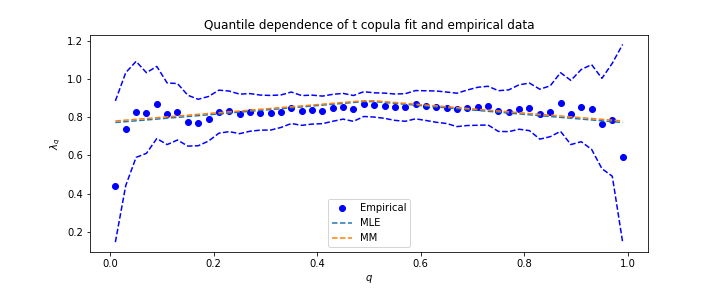
\includegraphics[width=\textwidth]{_pics/t Copula quantile dependence.png}
%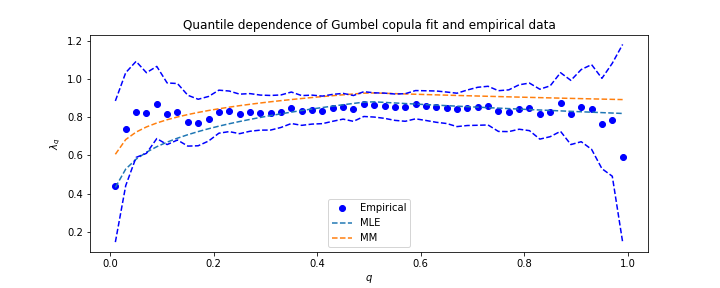
\includegraphics[width=\textwidth]{_pics/Gumbel Copula quantile dependence.png}
%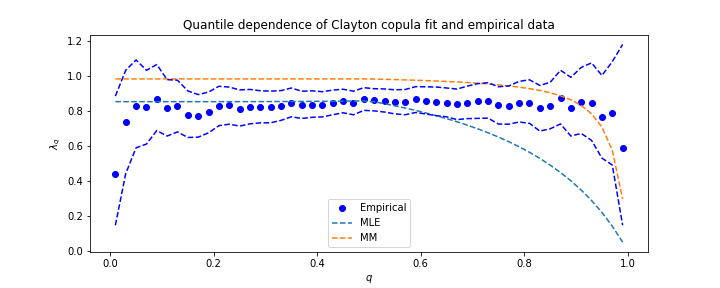
\includegraphics[width=\textwidth]{_pics/Clayton Copula quantile dependence.png}
%  \caption{}
%\label{fig:quantile dependence1}
%\end{figure}


The MM estimation perform just as we decided: match the upper and lower quantile dependence.




%
%
%\subsection{Two-Stage Estimation}\label{subsec:two-stage-estimation}
%~\cite{joe2005asymptotic} study the efficiency of a two-stage estimation procedure of copula estimation.
%The authors also call this method inference function for margins IFM.
%
%\textbf{Pros}
%\begin{enumerate}
%    \item Almost as efficient as MLE methods but easier to be implemented
%    \item Yields an asymptotically Gaussian, unbiased estimate
%\end{enumerate}
%
%\textbf{Cons}
%\begin{enumerate}
%    \item Subject to specification of marginals \cite{kim2007comparison}
%\end{enumerate}
%
%Our data
%\begin{align}
%    \pmb{y} = \begin{bmatrix}
%                  y_{11} & \cdots & y_{1i}\\
%                  \vdots & \ddots & \vdots \\
%                  y_{n1} & \cdots & y_{ni}
%                  \end{bmatrix}
%    \end{align}
%Let $F$ and $f$ be the joint cdf and joint density of $\pmb{y}$ with parameters $\pmb{\delta}$,
%and let $F_i$ and $f_i$ be the marginal cdf and marginal density for the $i^\text{th}$ random variable with parameters $\pmb{\theta}_i$, we have
%\begin{align}
%    f(\pmb{y}; \pmb{\theta}_1, \pmb{\theta}_2,\dots \pmb{\theta}_i, \pmb{\delta}) =
%    c\{F_1(\pmb{y}_1;\pmb{\theta}_1), F_2(\pmb{y}_2; \pmb{\theta}_2), \dots, F_i(\pmb{y}_1;\pmb{\theta}_i); \pmb{\delta}\}
%    \prod^i_{j=1}f_i(\pmb{y}_j;\pmb{\theta}_j)
%    \end{align}
%
%For a sample of size $n$, the log-likelihood of functions of the $i^\text{th}$ univariate margin is
%\begin{align}
%    L_i(\theta_i) = \sum^n_{m=1} \log f_i(y_{mi}; \theta_i),
%    \end{align}
%
%and the log-likelihood function for the joint distribution is
%\begin{align}
%    L(\delta, \theta_1, \theta_2, \dots, \theta_i) = \sum^n_{m=1}\sum^i_{j=1} \log f(y_{mj}; \delta, \theta_1, \theta_2, ..., \theta_i)
%    \end{align}
%
%In most cases, one does not have closed form estimators and numerical techniques are needed.
%Numerical ML estimation difficulty increase when the total number of parameters increases.
%The two-stage estimation is designed to overcome this problem.
%
%The two-stage procedure is
%\begin{enumerate}
%    \item estimate the univariate parameters from separate univariate likelihoods to get $\tilde{\pmb{\theta}_1}, ..., \tilde{\pmb{\theta}_i}$
%    \item maximize $L(\pmb{\delta}, \tilde{\pmb{\theta}_1}, \dots, \tilde{\pmb{\theta}_i})$ over $\pmb{\delta}$ to get $\tilde{\pmb{\delta}}$
%    \end{enumerate}
%
%Under regularity conditions
%\footnote{Regularity conditions include
%1. $\exists \frac{\partial \log f(x;\theta)}{\partial \theta}, \frac{\partial^2 \log f(x;\theta)}{\partial \theta^2}, \frac{\partial^3 \log f(x;\theta)}{\partial \theta^3}$ for all $x$;
%2. $\exists g(x), h(x) and H(x)$ such that for $\theta$ in a neighborhood $N(\theta_0)$ the relations
%$\left|\frac{\partial f(x;\theta)}{\partial theta}\right| \leq g(x)$,
%$\left|\frac{\partial^2 f(x;\theta)}{\partial \theta^2}\right| \leq h(x)$,
%$\left|\frac{\partial^3 f(x;\theta)}{\partial \theta^3}\right| \leq H(x)$ hold for all $x$, and
%$\int g(x) dx < \infty$, $\int h(x) dx < \infty$, $\mathbb{E}_\theta \{H(X)\} < \infty$ for $\theta \in N(\theta_0)$;
%3. For each $\theta \in \Theta$, $0< \mathbb{E}_\theta \left\{
%\left(
%\frac{\partial \log f(X;\theta)}{\partial \theta}
%\right)^2
%\right\}$. For detail see section 4.2.2 of~\cite{serfling2009approximation}}
%, $(\pmb{\tilde{\theta}}_1,\dots \pmb{\tilde{\theta}}_i, \pmb{\tilde{\delta}})$ is the solution of
%\begin{align}
%    (\partial L_1 / \partial \pmb{\theta}^\intercal_1,
%    \dots, \partial L_i / \partial \pmb{\theta}^\intercal_i, \partial L / \partial \pmb{\pmb{\delta}}^\intercal_1) = \pmb{0}
%    \end{align}
%
%For comparison, if we optimize $L$ directly without the two-stage procedure (i.e.~MLE), we solve for
%\begin{align}
%    (\partial L / \partial \pmb{\theta}^\intercal_1,
%    \dots, \partial L / \partial \pmb{\theta}^\intercal_i, \partial L / \partial \pmb{\pmb{\delta}}^\intercal_1) = \pmb{0}
%    \end{align}
%
%We denote the two solutions as
%$\tilde{\pmb{\eta}} = (\pmb{\tilde{\theta}}_1,\dots \pmb{\tilde{\theta}}_i, \pmb{\tilde{\delta}})$ for two-stage procedure;
%$\hat{\pmb{\eta}} =(\pmb{\hat{\theta}}_1,\dots \pmb{\hat{\theta}}_i, \pmb{\hat{\delta}})$ for MLE procedure.
%and compare the asymptotic relative efficiency of $\tilde{\pmb{\eta}}$ and $\hat{\pmb{\eta}}$.
%
%Asymptotics: yet to be done.\\
%~\cite{kim2007comparison} show the estimation of $\pmb{\theta}$ may be seriously affected.
%They compare the two-stage approach and Canonical Maximum Likelihood Method by simulation and
%conclude that Canonical Maximum Likelihood is prefered from a computational statistics and data analysis point of view.
%
%\subsection{Canonical Maximum Likelihood Method}\label{subsec:canonical-maximum-likelihood-method}
%This approach was studied by~\cite{genest1995semiparametric} and~\cite{shih1995inferences}.
%One estimates the margins using empirical CDF
%\begin{align}F_X(x)=\frac{1}{n+1}\sum_{i=1}^n 1(X_i \leq x)\end{align},
%
%we maximize the log-likelihood
%\begin{align}
%    L(\delta) = \sum_{i=1}^n \log [c_\delta \{F_X(X_i), F_Y(Y_i)\}]
%    \end{align}
%
%This procedure does not require specification of marginals.
%
%
%
%
%
%%also by Wang and Ding, 2000; Tsukahara, 2005
%%This is also known as pseudo maximum likelihood (PML) and as canonical maximum likelihood (see Cherubini et al., 2004)
%%
%%Genest and Werker (2002) obtained conditions under which the PMLE is asymptotically efficient.
%%
%%



\newpage
\bibliographystyle{abbrvnamed} %
\bibliography{finance} %
\end{document}

%%% Local Variables: 
%%% mode: latex
%%% TeX-master: t
%%% End: 
